\subsection{La lagrangiana di interazione.}
\subsection{Il cervello come ricevitore principale.}
\subsection{Il cuore come modulatore.}
\subsection{La relazione complementare.}

\subsection{La misura di \texorpdfstring{$\Phi$}{Phi}: corteccia versus cervelletto}
Il postulato 2 afferma che è la geometria della rete, e non il numero di neuroni, a determinare la ricezione. Per rendere l'affermazione verificabile numericamente, ho implementato un proxy maneggevole di $\Phi$: la divergenza di Kullback--Leibler tra il modello completo e il modello in cui i collegamenti che attraversano un taglio vengono rimossi, minimizzata su tutte le biparizioni, su dinamica di Glauber. Non è il $\Phi$ esatto dell'IIT 3.0; è un'approssimazione con la stessa firma ordinale.

\begin{table}[H]
\centering
\begin{tabular}{@{}cccc@{}}
\toprule
Unità & $\Phi$ corteccia & $\Phi$ cervelletto & Rapporto \\ \midrule
4 & $0,243 \pm 0,063$ & $0,012 \pm 0,014$ & 20,6 \\
6 & $0,259 \pm 0,049$ & $0,045 \pm 0,015$ & 5,8 \\
8 & $0,245 \pm 0,042$ & $0,036 \pm 0,030$ & 6,9 \\ \bottomrule
\end{tabular}
\caption{$\Phi$ per reti ricorrenti e feedforward, mediato su quattro reti casuali per dimensione.}
\label{tab:phi}
\end{table}

La rete ricorrente integra da 2 a 20 volte di più di quella feedforward a parità di unità. La conclusione qualitativa della versione 30 è quindi sostenuta numericamente, entro i limiti del proxy.

\begin{figure}[H]
\centering
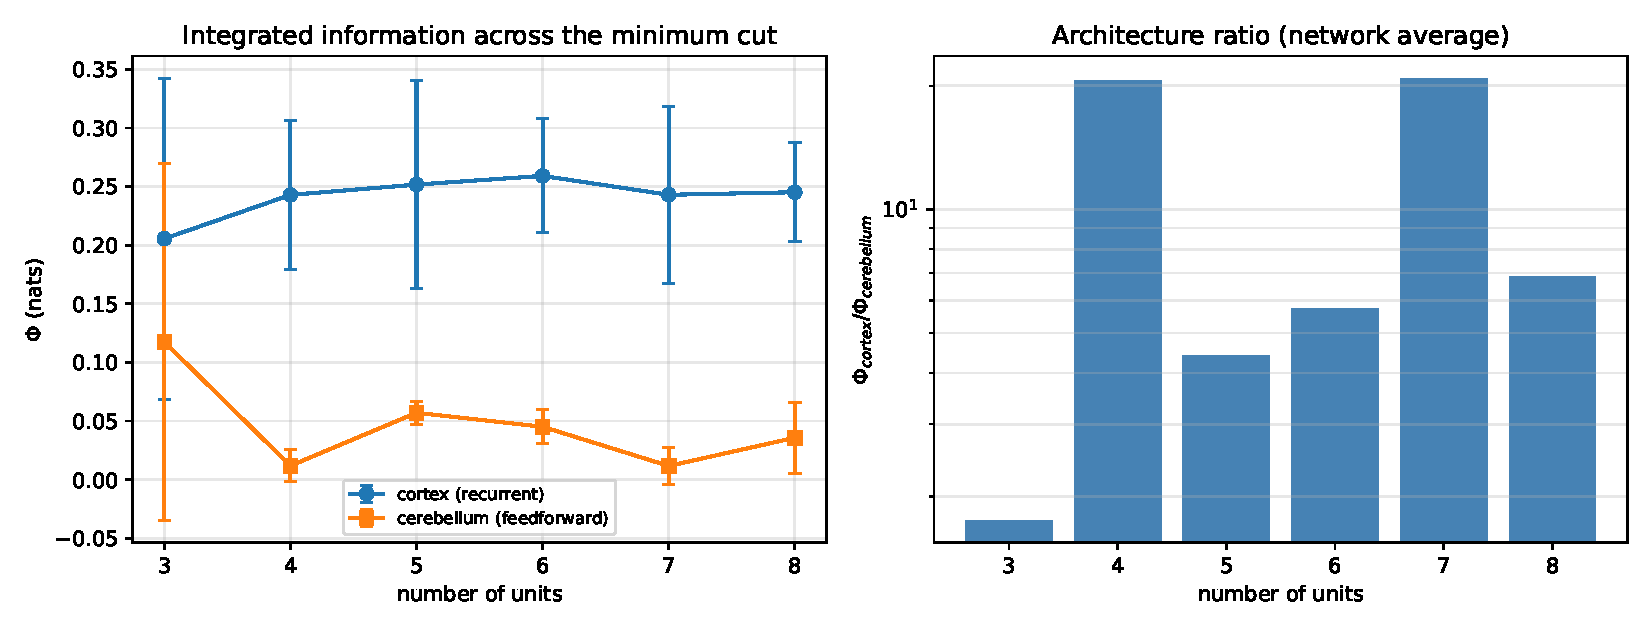
\includegraphics[width=0.9\textwidth]{figures/fig03_phi_architecture.pdf}
\caption{$\Phi$ per le due architetture, con deviazione standard su quattro reti casuali, e il rapporto tra esse.}
\label{fig:phi}
\end{figure}

\section{La derivazione dell'accoppiamento di Yukawa}
\subsection{Il meccanismo.}
\subsection{La stima (sviluppata):} La formula generale è $g_A \sim (M_4/M_{12})^5$. Per ottenere un valore numerico supponiamo che la scala di compattificazione sia $M_{12} \sim 10^{19}$ GeV (la scala di Planck) e che la scala elettrodebole sia $M_4 \sim 10^3$ GeV. Allora:
\begin{equation}
g_A \sim \left(\frac{10^3}{10^{19}}\right)^5 = (10^{-16})^5 = 10^{-80}
\end{equation}
Questo valore è estremamente piccolo, il che significa che l'accoppiamento è molto debole. Va sottolineato che i fattori di sovrapposizione tra le funzioni d'onda dei modi KK e le brane non possono elevare il valore effettivo a $\sim 10^{-3}$: la sovrapposizione di funzioni d'onda normalizzate è al massimo 1, quindi servirebbe un fattore di $10^{77}$, il che è impossibile. Il valore adottato in questo articolo è dunque $g_A \sim 10^{-80}$.

Questo valore è anche l'unico compatibile con i dati. Se il campo si accoppiasse alla Yukawa ai nucleoni, la forza relativa alla gravitazione sarebbe
\begin{equation}
\alpha = \frac{g_A^2\, \hbar c}{G\, m_p^2} = g_A^2 \times 1,69\times10^{38}.
\end{equation}
Per $g = 10^{-3}$ risulterebbe $\alpha \approx 1,7\times10^{32}$, escluso dai test di laboratorio di circa 35 ordini di grandezza. Il vincolo del 7\% citato nell'introduzione implica $g < 2\times10^{-20}$. Inoltre un accoppiamento $g = 10^{-3}$ darebbe al modo una vita media dell'ordine di $10^{-3}$ s, incompatibile con la stabilità della materia oscura. La stima $g_A \sim 10^{-80}$ rende quindi la teoria predittiva e non solo coerente.
\subsection{Lo schermaggio di Debye.}
\subsection{La forza effettiva.}

\section{I tachioni come intermediari}
\subsection{Lo spettro tachionico:} $m_n^2 = n^2/R^2 - \mu_A^2$.
\subsection{L'accoppiamento tachionico.}
\subsection{La relazione bradione--tachione.}
\subsection{Che cosa trasportano i tachioni.}

\section{I vuoti del campo akashico}
\subsection{Che cos'è un vuoto?}
\subsection{I tre tipi di vuoto.}
\subsection{Il vuoto del campo akashico.}
\subsection{Più vuoti.}

\section{La dualità onda--particella}
\subsection{Il meccanismo in quattro fasi.}
\subsection{Che cosa trasporta l'onda.}
\subsection{L'analogia dell'albero.}

\section{Le equazioni del moto complete}
\subsection{L'equazione akashica.}
\subsection{L'equazione della coscienza.}
\subsection{L'equazione dei bosoni esotici.}
\subsection{L'equazione di Einstein in 12D.}

\newpage
